\chapter{Propaedeuticum: Fundamental Considerations of Deep Neural Networks}
To form a basis for the thesis, a toy problem is used to exemplify the conceptual idea of the functioning of an Artificial Neural Network (NN). To understand the mathematical background especially probabilistic considerations are introduced. For the technical background the use of a Python library for machine learning called PyTorch \cite{Paszke2019Dec} is presented.

\section{Toy Problem}
The example multivariate data set \cite{Dua:2019} is taken from Python's Scikit-learn package \cite{pedregosa2011scikit}. It contains chemical analyses of two types of wine of $130$ wines grown in the same region in Italy. In total $13$ components were analyzed that appeared in both wines, such as the alcohol or magnesium content. In the following, these are called features. Originally, the data set contained three wine varieties, but since the toy problem was to be kept as simple as possible, the data for the third wine type was removed. The toy problem is to develop a NN that can match a wine sample to the correct variety based on the $13$ features.

The distribution of the feature \textit{alcohol content} of all samples is exemplary visualized in Fig. \ref{fig:alcohol_freq}: Samples of the variety labeled with $1$ have a mean of 12.3 vol\% and standard deviation 0.5 vol\%, while the samples of the wine with target $0$ have a significantly higher mean value (13.8 vol\%) and scatter less.

Looking at e.g. the bivariate data set of the features alcohol and magnesium content, no linear correlation is apparent (Fig. \ref{fig:corr_wine}).
\begin{figure}
	\centering
	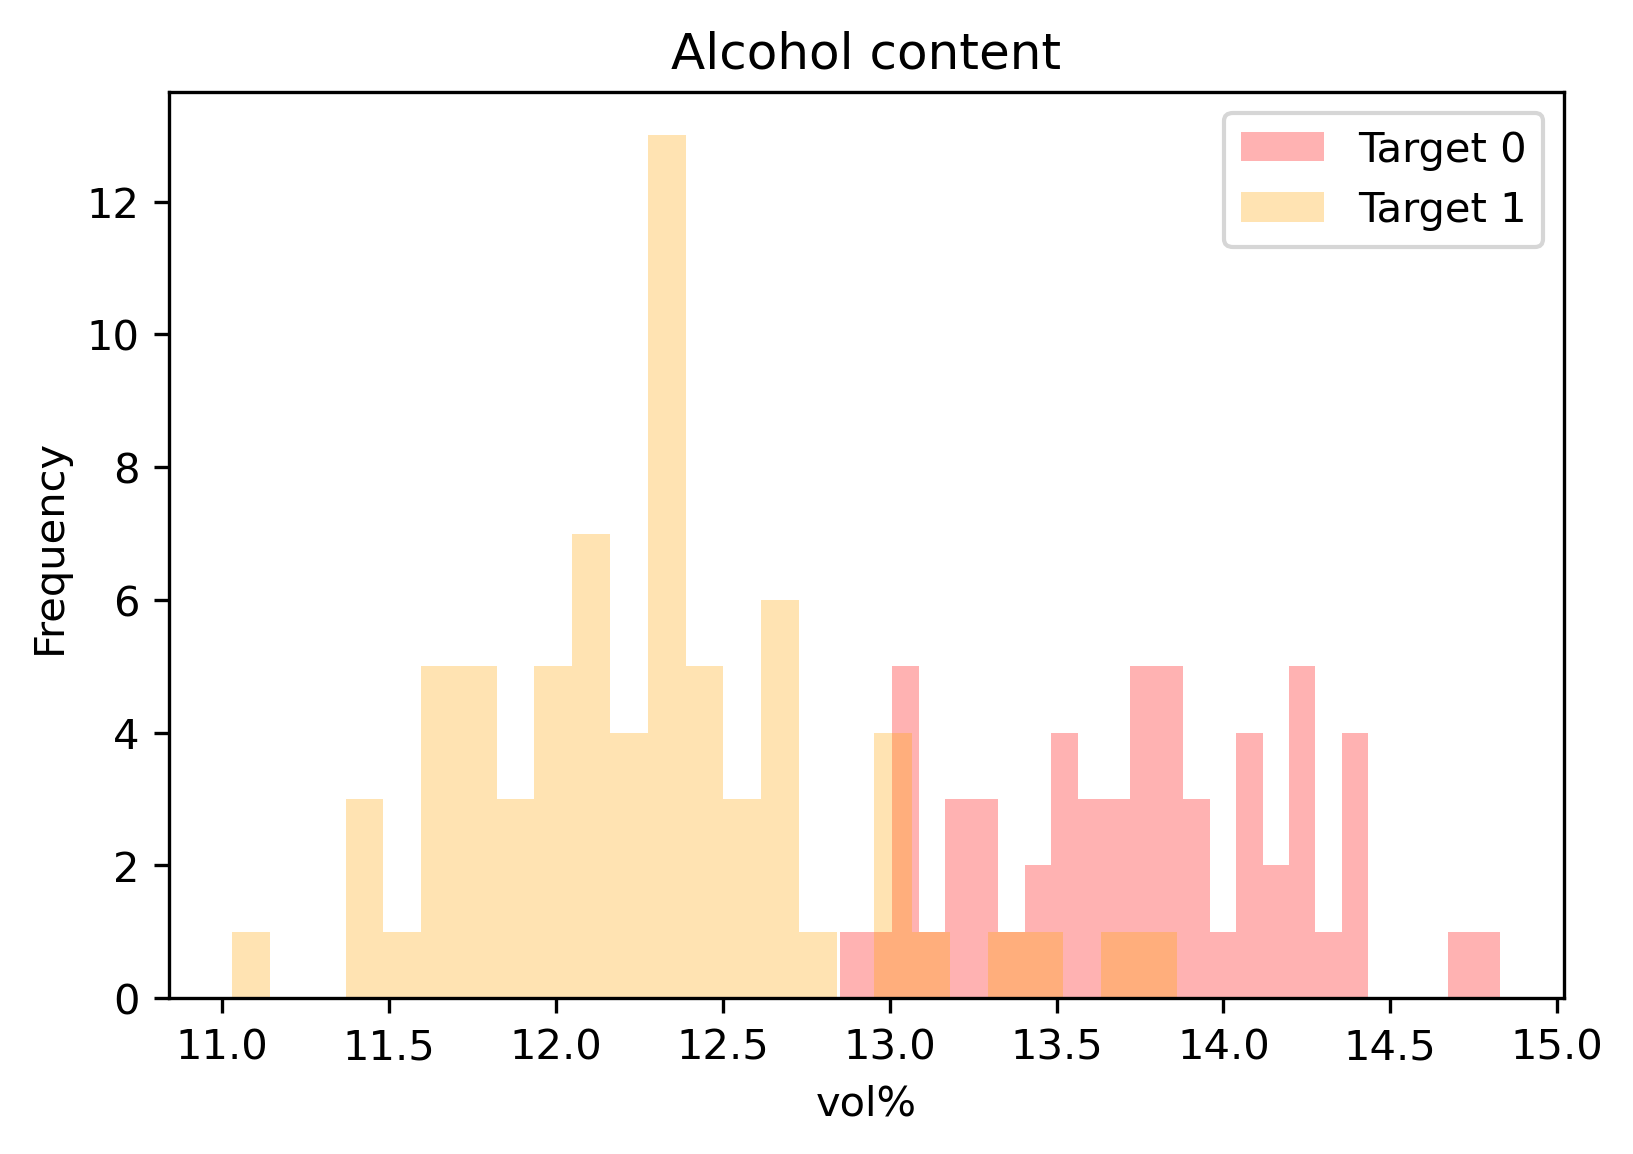
\includegraphics[scale=0.7]{images/alcohol_freq.png}
\caption{Absolute alcohol frequencies of wines in the wine data set.}
\label{fig:alcohol_freq}
\end{figure}

\begin{figure}
	\centering
	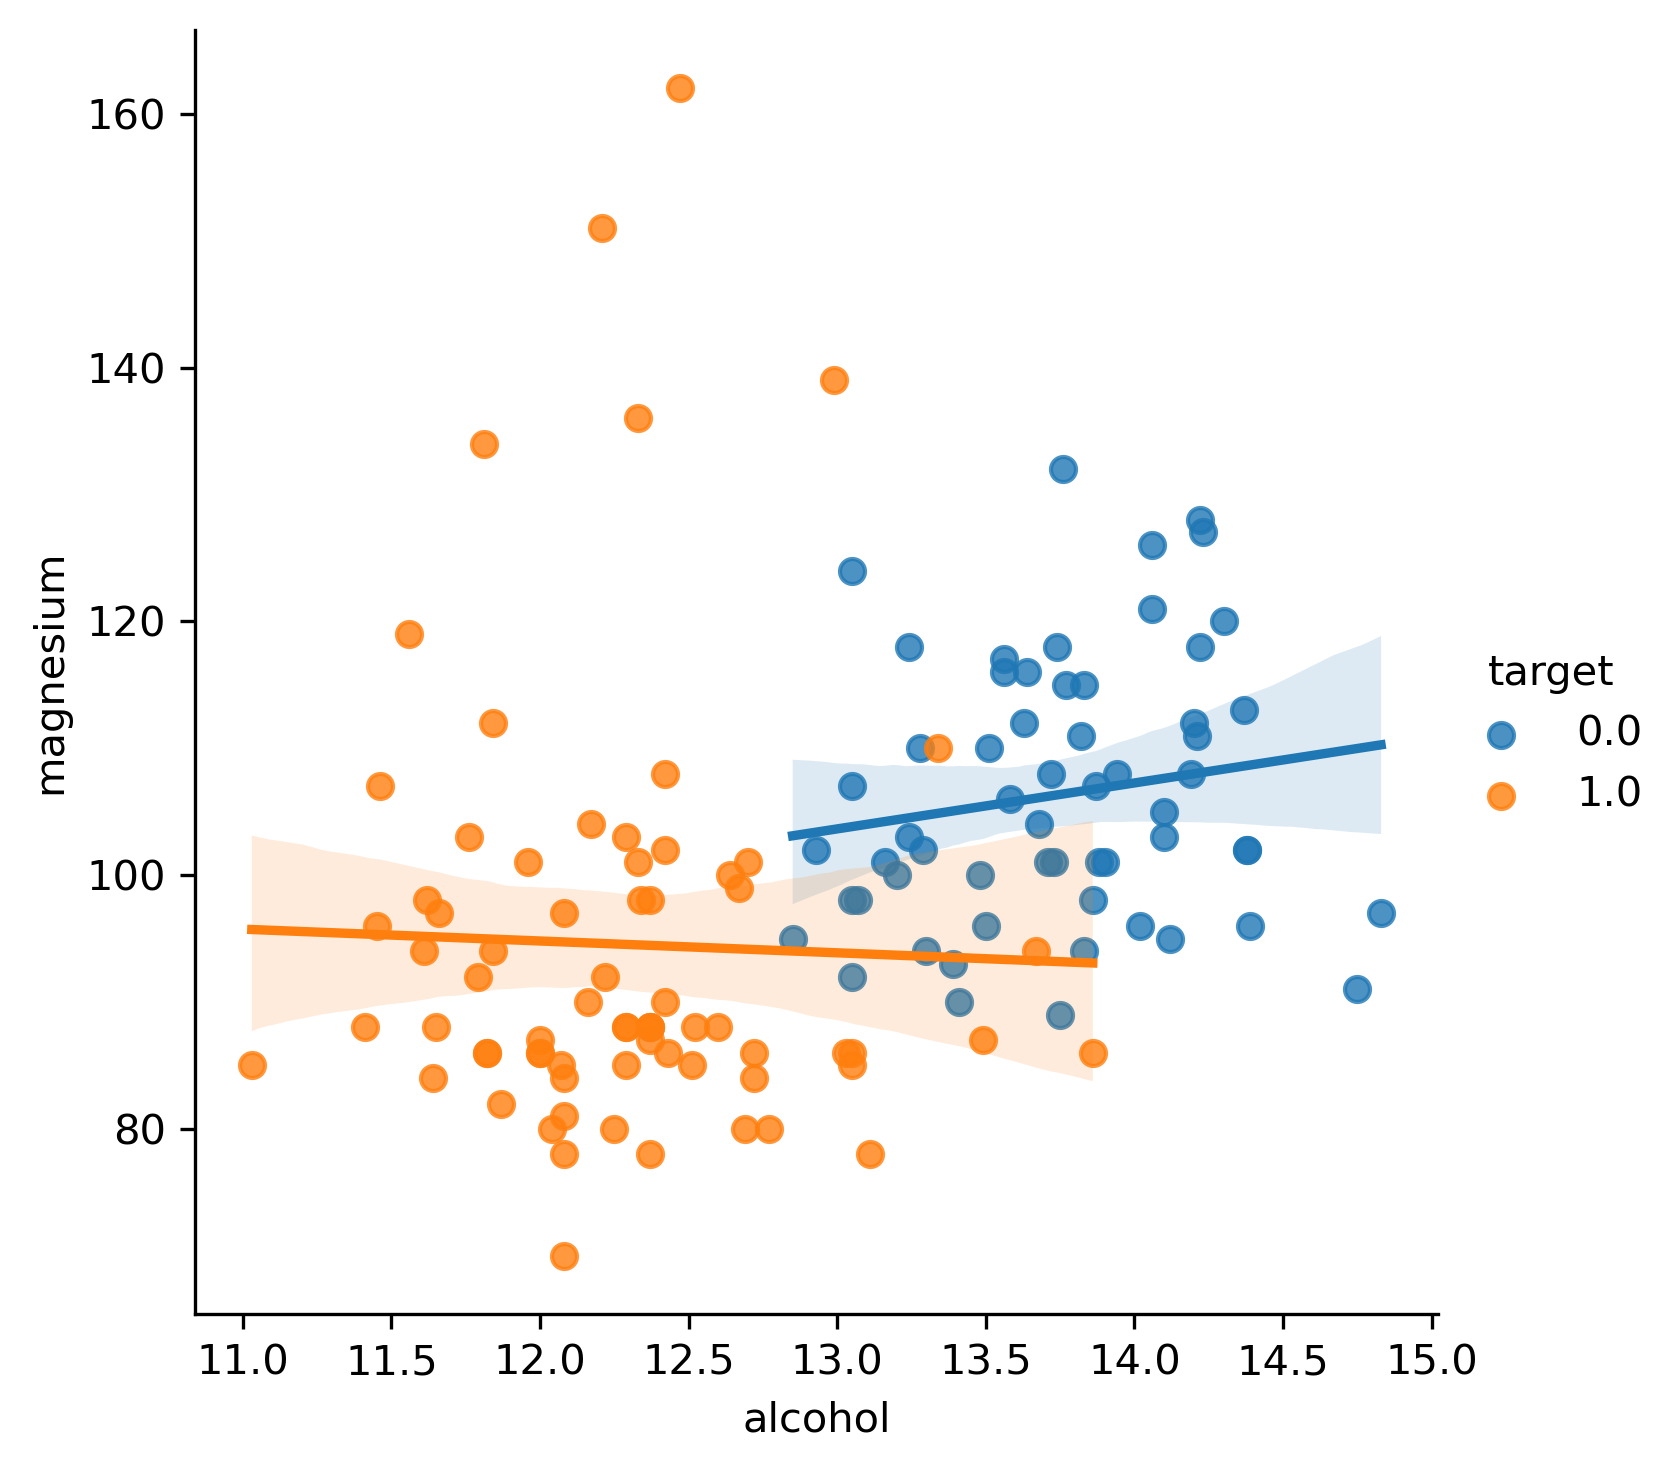
\includegraphics[scale=0.18]{images/corr_wine.png}
\caption[Regression of 2 wine data set features]{Bivariate considerations between alcohol content [vol\%] and magnesium content [mg]: Linear regression with 95\% confidence interval.}
\label{fig:corr_wine}
\end{figure}


\section{Definitions and Mathematical Background}
In order to embed the operating principle of a NN with more than one hidden layer, which is a so-called Deep Neural Network (DNN), in a mathematical and, in particular, probabilistic context, a basic mathematical notion must first be defined, which is inspired by Goodfellow et al. \cite{Goodfellow-et-al-2016}.

\textbf{Fundamentals of Probability Theory}\\
A random variable (RV) $X$ is formally a measurable mapping that assigns elements from a probability space to elements of a measurable space. Where a measurable space, by definition consists of a basic set over which a $\sigma$ - algebra is defined. A probability space is a measure space which is, compared to a measurable space provided with a probability measure. Due to inverse image and probability measure properties, a measure is also defined on the image of $X$, which makes the measurable image space to a measure space.

According to the definition of the counting densities, each discrete probability measure has a probability density with respect to the counting measure, this is also known as probability mass function (PMF) and provides possible values and the associated probabilities of a discrete RV.

Probability measures whose distribution functions are continuous, are absolutely continuous with respect to the Lebesgue measure, therefore, according to the Radon-Nikodym theorem, there exists a so called probability density function (PDF). The Lebesgue integral (and with corresponding theorems also the Riemann integral) of this function over a set of the probability space corresponds to the probability of the RV to assume values in this set.

In order not to go beyond the scope of this Propaedeuticum, the following simplifying assumptions for RV are made:
\begin{enumerate}
    \item A RV $\vec{X}$ can either be discrete-valued: $\vec{X}\in\{\vec{x_1}, \vec{x_2}, ...\}$, or continuous-valued: $\vec{X} \in \mathbb{R}^d$
    \item If $\vec{X}$ is discrete-valued, $\vec{X}$ has a PMF $P$: $\vec{X} \sim P(\vec{X} = \vec{x_i}) = P({x_i}) = p_i \geq 0$, where $p_i$ is the probability that $\vec{X} = \vec{x_i}$.
    \item If $\vec{X}$ is continuous-valued $\vec{X}$ has a PDF $p$: $\vec{X} \sim p(\vec{x}) \geq 0$
\end{enumerate}
Due to properties of the probability measure, the sum of all $p_i$ of a RV or the integral over the PDF of a RV equals $1$.

Using the Dirac function $\delta$, a PDF $\hat{p}$ for a discrete-valued RV can also be set up:
\begin{equation}
    \hat{p}(\vec{x}) = \sum_{i} p_i \delta(\vec{x}-\vec{x_i}).
    \label{eq:disc}
\end{equation}
At this place it should be pointed out for completeness that the Dirac function is formally a (regular) distribution, hence a linear, continuous functional, which assigns functions from the space of test functions, e.g. the space of infinitely often differentiable functions with compact support, to a real (or complex) number.

Let $\vec{X} \sim p(\vec{x})$, and $\vec{Y} \sim p(\vec{y})$ be RV with corresponding PDFs then the following can be defined:

\begin{definition}[Expectation value]
\begin{equation}
    \mu := E(\vec{X}) := \int_{-\infty}^{\infty} \vec{x} p(\vec{x})\mathrm{d}\vec{x}
\end{equation}
\end{definition}

\begin{definition}[Joint distribution]
The Joint distribution is the vertically stacked PDF:
\begin{equation}
    p(\vec{x},\vec{y}) := 
    p\Biggl(\begin{pmatrix}\vec{x}\\\vec{y}\end{pmatrix}\Biggr)
\end{equation}
\end{definition}

\begin{definition}[Marginal distribution]
The marginal distribution is the integral of the joint distribution of one RV:
\begin{align}
    p(\vec{x}) = \int p(\vec{x},\vec{y})\mathrm{d}\vec{y} \\
    p(\vec{y}) = \int p(\vec{x},\vec{y})\mathrm{d}\vec{x}
\end{align}
\end{definition}

\begin{definition}[Conditional distribution]
\begin{align}
    p(\vec{x}|\vec{y}) := \frac{p(\vec{x},\vec{y})}{p(\vec{y})} \\
    p(\vec{y}|\vec{x}) := \frac{p(\vec{x},\vec{y})}{p(\vec{x})}
    \label{eq:cond}
\end{align}
\end{definition}

To measure the dissimilarity between two PDFs $p$ and $q$ the Kulback-Leibler divergence and cross entropy can be used.
\begin{definition}[Kullback-Leibler divergence]
Let $p$ and $q$ be two PDFs then the Kullback-Leibler divergence  (KLD) \cite{Kullback1951Mar} is defined as:
\begin{equation}
    D_{KL}(p \parallel q) := \int p(\vec{x}) \cdot \ln\biggl(\frac{p(\vec{x})}{q(\vec{x})}\biggr)\mathrm{d}\vec{x} = E_{\vec{X} \sim p} \biggl[\ln\biggl(\frac{p(\vec{x})}{q(\vec{x})}\biggr)\biggr],
\end{equation}
\end{definition}
where $E_{\vec{X}\sim p}$ is the expectation value according to $p$.

It can be shown that:
\begin{enumerate}
    \item $D_{KL}(p \parallel q) \geq 0$
    \item $D_{KL}(p \parallel q) = 0 \Leftrightarrow p = q$
    \item $D_{KL}(p \parallel q) \neq D_{KL}(q \parallel p)$.
    \label{eq:prop_KL}
\end{enumerate}
\begin{definition}[Entropy]
The entropy of a probability distribution $p$ is defined as:
\begin{align}
    H(p) := -\int p(\vec{x})\ln(p(\vec{x}))\mathrm{d}\vec{x}
\end{align}
\end{definition}

\begin{definition}[Cross entropy]
The cross entrpopy (CE) between two different probability distributions $p$ and $q$ is defined as:
\begin{align}
    H(p,q) := -E_{\vec{X}\sim p} \left[\ln(q(\vec{x}))\right] = - \int_{-\infty}^{\infty}p(\vec{x})\ln(q(\vec{x}))\mathrm{d}\vec{x} \geq 0
\end{align}
\end{definition}

It holds by definition
\begin{equation}
D_{KL}(p \parallel q) = \int p(\vec{x}) \ln\biggl(\frac{p(\vec{x})}{q(\vec{x})}\biggr) \mathrm{d}\vec{x} \overset{\text{Log. rules}}{=} \underbrace{\int p(\vec{x}) \ln(p(\vec{x}))\mathrm{d}\vec{x}}_{=\:-H(p)} \underbrace{- \int p(\vec{x}) \ln(q(\vec{x})) \mathrm{d}\vec{x}}_{=\:H(p,q)}.
\label{eq:DKL_CE}
\end{equation}
With eq. \ref{eq:DKL_CE} and properties of the KLD we have
\begin{align}
    H(p,q) = \underbrace{D_{KL}(p\parallel q)}_{\geq 0} + H(p) \geq H(p) \geq 0.
\end{align}
For fixed $p$ follows
\begin{align}
    \min_q D_{KL} (p \parallel q) \Leftrightarrow \min_q H(p,q).
    \label{eq:optim_CE}
\end{align}
Thus minimizing KLD or CE results the same. 

All considerations made for RV with continuous PDFs can also be applied to discrete RV, by changing the integral into a sum.
\\
\\
\textbf{Probabilistic Framework of Supervised Learning}
\begin{definition}[Bayes rule]
\begin{equation}
    \underbrace{p(\vec{y}|\vec{x})}_{posterior} = \underbrace{p(\vec{x}|\vec{y})}_{likelihood} \cdot \frac{\overbrace{p(\vec{y})}^{prior}}{\underbrace{p(\vec{x})}_{evidence}}
\end{equation}
\end{definition}
Based on Bayes' theorem, in Bayesian estimation theory with known likelihood, prior, and evidence, a posterior density function (posterior) can be calculated.

In NNs likelihood and prior are unknown. Therefore, we try to approximate posterior $p(\vec{x}|\vec{y})$ by a PDF $q(\vec{x}|\vec{y}; \vec{\theta})$. The PDF $q$ is given by the architecture of the NN. Only the parameters $\vec{\theta}$ have to be learned using a training data set and KLD/CE as measure for dissimilarity of $p$ and $q$. Finding a PDF as close as possible to $p$ turns out into an optimization problem. The goal is to minimize CE by changing $\vec{\theta}$. First the CE should only be dependent on $\Vec{\theta}$ and has to be reformulated as
\begin{align}
    H(p(\vec{x},\vec{y}), q(\vec{x},\vec{y}; \vec{\theta})) \overset{\text{Def.}}&{=} - \int p(\vec{x},\vec{y}) \ln{q(\vec{x},\vec{y};\vec{\theta})}\mathrm{d}\vec{x}\mathrm{d}\vec{y} \nonumber\\ 
    \overset{\ref{eq:cond}}&{=} - \int p(\vec{x},\vec{y}) \ln{q(\vec{y}|\vec{x};\vec{\theta})}\mathrm{d}\vec{x}\mathrm{d}\vec{y} - \underbrace{\int p(\vec{x},\vec{y}) \ln{q(\vec{x})}\mathrm{d}\vec{x}\mathrm{d}\vec{y}}_{:=\: c\in \mathbb{R}} \nonumber\\
    &= \int p(\vec{x},\vec{y}) [-\ln{q(\vec{y}|\vec{x};\vec{\theta})}]\mathrm{d}\vec{x}\mathrm{d}\vec{y} + c.
    \label{eq:minH_00}
\end{align}
Thus, the joint distribution can be represented according to eq. \ref{eq:cond} as the product of conditional and marginal distribution, and the second summand in the upper equation is constant because it is independent of $\vec{\theta}$.\\
In the toy problem one sample consists of 13 features thus $\vec{x}\in \mathbb{R}^{13}$ and
\begin{equation}
 \vec{y} \in \biggl\{\left(\begin{array}{c} 1 \\ 0 \end{array}\right), \left(\begin{array}{c} 0 \\ 1 \end{array}\right)\biggr\}.
 \label{eq:hot_coding}
\end{equation}
 labels the corresponding wine variety $0$ or $1$.  Let $\vec{e_1}$ stand for variety $0$ and $\vec{e_2}$ for wine variety $1$. This type of labeling is also referred to as one-hot-coding and will be needed later.
 \\
 \\
 The training data set contains finite samples $\vec{x}$ with corresponding wine variety $\vec{y}$ (supervised learning). Each sample $j$ is uniformly distributed with $p_j = \frac{1}{N}$, where $N$ is the size of the training data set. Thus, the unknown joint distribution $p(\vec{x},\vec{y})$ is given with eq. \ref{eq:disc} to
\begin{equation}
    \hat{p}(\vec{x},\vec{y}) = \frac{1}{N} \sum_{j=1}^N \delta(\vec{x}-\vec{x}(j),\vec{y}-\vec{y}(j)),
    \label{eq:sample_distr}
\end{equation}
where the term $\delta(\vec{x}-\vec{x}(j),\vec{y}-\vec{y}(j))$ equals 1 for a corresponding sample because of properties of the Dirac function.
\\
For the minimization problem, it follows with eqs. \ref{eq:minH_00} and \ref{eq:sample_distr}
\begin{align}
    \min_{\vec{\theta}} H(\hat{p},q) = \int \frac{1}{N} \sum_{j=1}^N \delta(\vec{x}-\vec{x}(j),\vec{y}-\vec{y}(j))[-\ln{q(\vec{y}|\vec{x};\vec{\theta})}]\mathrm{d}\vec{x}\mathrm{d}\vec{y} + c.
\end{align}
Since in the integral, due to the Delta function only null sets are left, it gets cancelled. The constant $c$ can be neglected at minimization of $\vec{\theta}$. Thus it holds
\begin{align}
    \min_{\vec{\theta}} H(\hat{p},q) &= \frac{1}{N} \sum_{j=1}^N \delta(\vec{x}-\vec{x}(j),\vec{y}-\vec{y}(j))[-\ln{q(\vec{y}|\vec{x};\vec{\theta})}] \nonumber\\
    &= \frac{1}{N} \sum_{j=1}^N \underbrace{[-\ln{q(\vec{y}(j)|\vec{x}(j);\vec{\theta}}]}_{=:\:  l(\vec{x}(j),\vec{y}(j);\vec{\theta})},
    \label{eq:min_CE_dis}
\end{align}
since the Delta function equals $1$ for each sample.

These transformations thus replace the unknown PDF $p$ with concrete training data points. Now, the so-called cost or loss function $L(\vec{\theta})$ can be optimized using a data set
\begin{equation}
    L(\vec{\theta}) = \frac{1}{N} \sum_{j=1}^N l(\vec{x}(j),\vec{y}(j);\vec{\theta}).
    \label{eq:coss}
\end{equation}

\section{Neural Network}
According to eq. \ref{eq:min_CE_dis}, an optimal $\vec{\theta}$ must be found to minimize $H(\hat{p},q)$. Or in other words, $p(\vec{y}|\vec{x})$ should be approximated by a model $q(\vec{y}|\vec{x};\theta)$. This is realized by creating a model or NN $f(\vec{x},\vec{\theta})$ learning $\vec{\theta}$ from training data by solving an optimization problem. In general NNs with enough layers and nonlinear activations can be considered as universal function approximators \cite{Cybenko1989Dec} and are able to learn every continuos relation over compact input sets \cite{Hornik1991Jan}.
\\
\\
\textbf{Preparation of Data}\\
After deleting entries of the third wine type in the data set as described above, target $\vec{y}$ and input vector $\vec{x}$, which are stored together in one 14 dimensional sample in the data set, were separated from each other. This was realized after reading the data set with basic Pandas Dataframe operations \cite{reback2020pandas}. With \texttt{train\_test\_split} from Sklearn the data set can randomly be split into training data and test data. In this function the parameter \texttt{train\_size} can be used to set the ratio of training data to test data. To avoid tight contour lines due to different orders of magnitude of each feature in the loss function, both training and test data were normalized with functions of Sklearn which improves the optimization. A detailed description of the normalization methods used is given in the documentation \cite{SKLEARN_DOC}.\\
\\
\textbf{Architecture of a Dense Neural Network}\\
Derived from biological neurons, also in artificial neurons, as the smallest unit of a DNN, information should be changed and passed on under certain conditions. A linear neuron can be described by a function with $d$ input signals $\Vec{x} = [x_1, ... ,x_d]^T \in\mathbb{R}^d$ with $d$ weights $\Vec{w} = [w_1, ... , w_d]^T \in \mathbb{R}^d$ and a bias or offset $b \in \mathbb{R}$. To model nonlinear relationships there can be added an additional activation function $\phi: \mathbb{R} \rightarrow \mathbb{R}$ to ultimately provide an output $y_{pred} \in \mathbb{R}$ to be calculated
\begin{equation}
    y_{pred} = \phi(\Vec{w}^T\Vec{x}+b).
\end{equation}
Several neurons are combined in one so-called layer. Each of the $d$ input entries is fully connected with $d$ neurons. $\Vec{w} \in\mathbb{R}^{d\times c}$ corresponds to the weight matrix and $\Vec{b}=[b_1, ... b_c]^T \in \mathbb{R}^c$ denotes the bias vector, where the layer consists of $c$ neurons. Since each neuron has one $y_{pred} \in \mathbb{R}$, the output of the layer is vector-valued. In a layer there are no interactions between the neurons. The $c\cdot d$ weights and $c$ biases are called parameters of a DNN, which are in the domain of the loss function and correspond to $\vec{\theta}$.

A so called feed forward DNN is the combination of several layers, where the output $\vec{y}_{pred}$ of the previous layer is used as input of the current layer.

For the toy problem, a small NN named \texttt{WineDecision} was built using PyTorch. PyTorch is an open source machine learning framework, that is particularly well suited for the creation of NNs due to its autograd system, GPU acceleration and high flexibility because of the usage of dynamic computation graphs \cite{Paszke2019Dec}. By inheriting PyTorch's \texttt{nn.Module}, functions implemented by the library can be used for the NN. In the constructor for this, first the constructor of the \texttt{nn.Module} class is called and then one \texttt{nn.Linear} layer provided by PyTorch is added to the \texttt{WineDecision} NN. It takes a \texttt{n\_input\_features} - dimensional input and maps it to a 1 dimensional output. Thus $d=13$ and $c=1$, since only one neuron is considered (Fig. \ref{fig:neuron}).\\
The input vector is first multiplied by the weights, the bias is added and then the \textit{sigmoid} function is applied to it, to finally return a $y_{pred}$. Depending on whether a forward or backward pass is executed, the derivative of each operation is calculated. In line 13 the model is initialized (Listing \ref{code:pytorch_NN_aufbau}).
\begin{lstlisting}[float, language=python, caption={Structure of one layer neural network with PyTorch.}, label=code:pytorch_NN_aufbau]
class WineDecision(nn.Module):

    def __init__(self, n_input_features: int):
        super(WineDecision, self).__init__()
        self.linear = nn.Linear(n_input_features, 1)

    def forward(self, x: torch.tensor):
        # constrain values (0 < y < 1)
        y_pred = torch.sigmoid(self.linear(x))
        return y_pred

# n_features = 13
model = WineDecision(n_features)
\end{lstlisting}
\begin{figure}
	\centering
	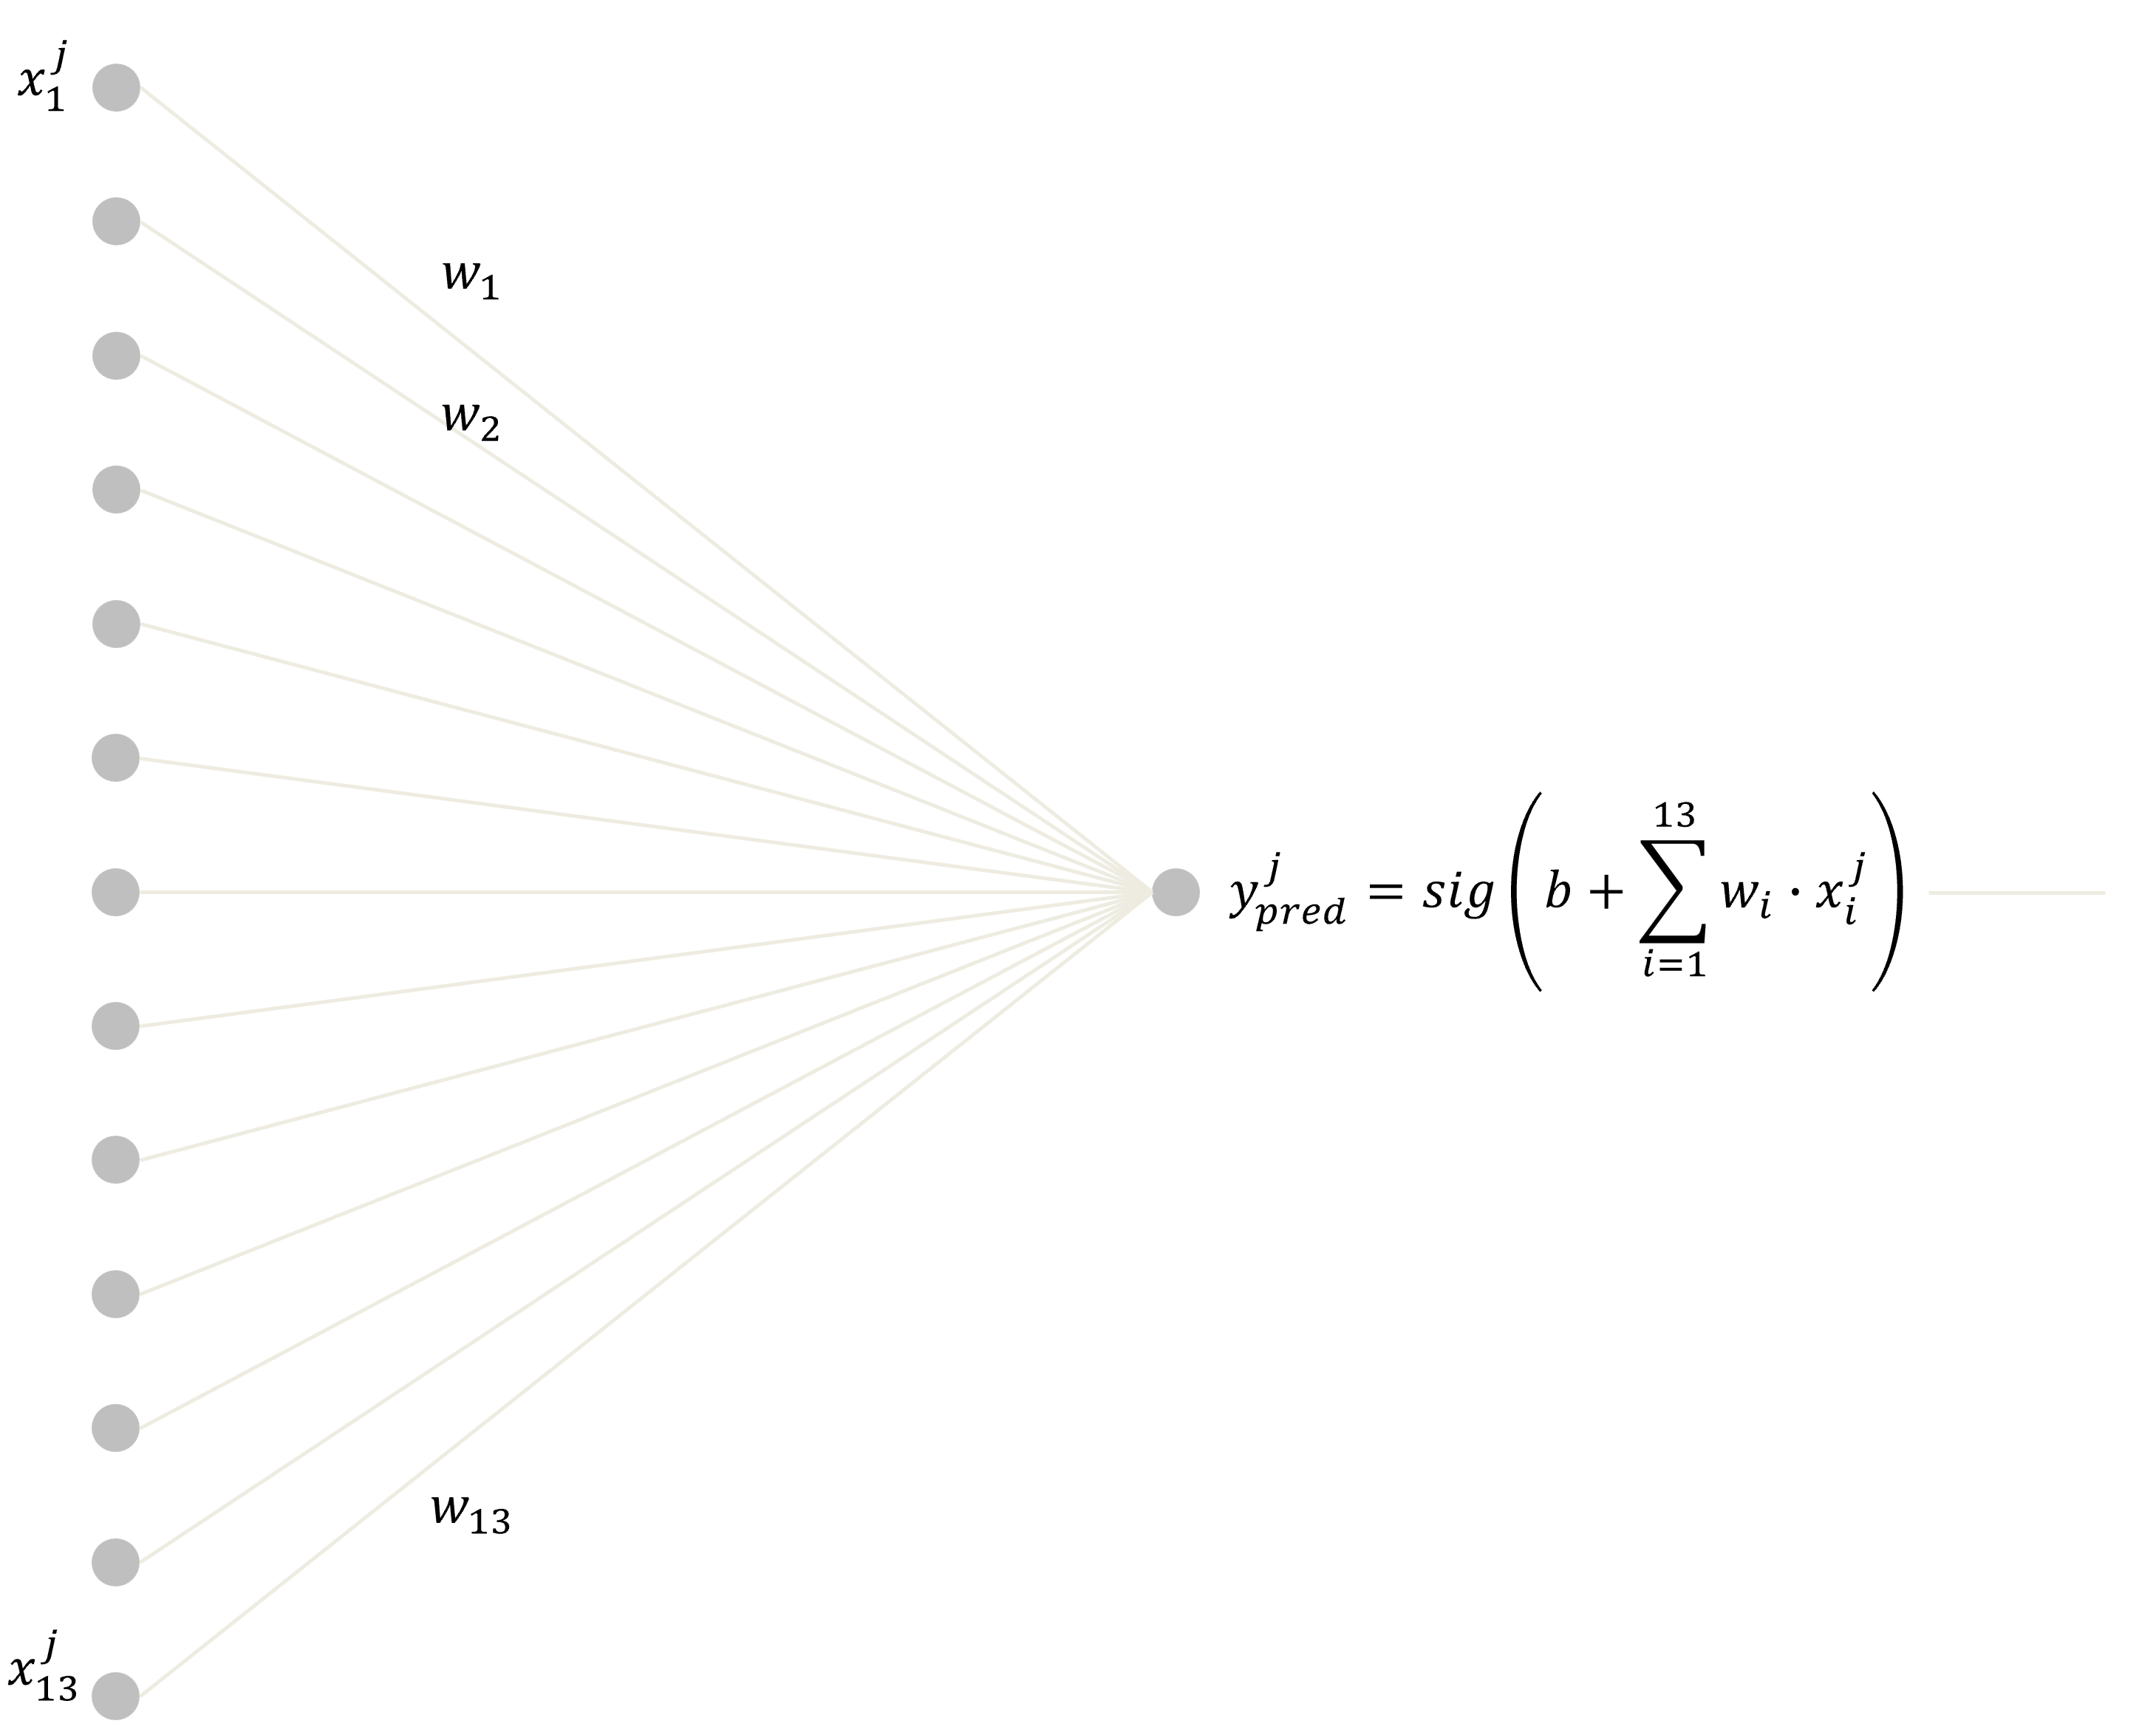
\includegraphics[scale=0.7]{images/neuron.png}
\caption[Example for a small NN]{Calculations of the small implemented \texttt{WineDecision} NN for one specific wine sample $j$ with its 13 features.}
\label{fig:neuron}
\end{figure}
The \textit{sigmoid} function
\begin{equation}
    sig(x) = \frac{1}{1+e^{-x}},
\end{equation}
has besides its nonlinearity another important property for the binary-classification toy problem: It only assumes values between $0$ and $1$. Usually higher order classification problems are realized with so-called softmax activation functions, for a binary-classification problem the simple sigmoid function is sufficient: If $y_{pred}$ takes values $\geq$ 0.5, the NN decides for wine type $1$ otherwise $0$.

\textbf{Loss Calculation}\\
With eq. \ref{eq:coss} the loss function to be optimized has already been introduced, but to be concretely applicable to the binary-classification toy problem, it still needs to be simplified.

The probability that given a sample $\vec{x}$, the wine belongs to the variety $0$ can be written with the notation of eq. \ref{eq:hot_coding} as
\begin{equation}
    p_1 = P(\vec{y}(j) = \vec{e_1}|\vec{x}(j)).
\end{equation}
$P$ is a posterior PMF that is unknown. In general, the probability that sample $j$ of $\vec{x}$ belongs to wine variety $0$ or $1$ can be written as
\begin{equation}
P(\vec{y}(j)|\vec{x}(j)) = p_1(j)^{y_1(j)} \cdot p_2(j)^{y_2(j)},
\end{equation}
where $y_1(j)$ is the first and $y_2(j)$ the second entry of $\vec{y}(j)$, respectively. Since a fixed wine sample $j$ cannot belong to two wine types at the same time, $y_1= 0$ if $y_2 = 1$ and vice versa. As mentioned at the beginning, the unknown $p_i(j)$ are approximated by $q_i(j)$ ($i \in \{1,2\}$) with a PMF $Q$. While $q_i(j)$ is approximated by a forward pass of the NN $f(\vec{x}(j);\theta)$. Thus holds
\begin{equation}
    Q(\vec{y}(j)|\vec{x}(j);\vec{\theta}) = f_1(\vec{x}(j);\vec{\theta})^{y_1(j)} \cdot f_2(\vec{x}(j);\vec{\theta})^{y_2(j)}.
    \label{eq:Qtof}
\end{equation}
In the binary classification problem holds
\begin{equation}
    f_1(\vec{x}(j),\vec{\theta}) = y_{pred}(\vec{\theta},j) \quad\qquad f_2(\vec{x}(j),\vec{\theta}) = 1-y_{pred}(\vec{\theta}, j),
    \label{eq:def_ypred}
\end{equation}
where $y_{pred}(\vec{\theta}, j)$ is the output of the \texttt{WineDecision} NN of one sample j. Then $l$ of eq. \ref{eq:coss} at a given sample $j$ is given by
\begin{align}
        l(\vec{x}(j),\vec{y}(j);\vec{\theta}) \overset{\ref{eq:min_CE_dis}}&{=} -\ln{Q(\vec{y}(j)|\vec{x}(j);\vec{\theta})} \nonumber\\
    \overset{\ref{eq:Qtof}}&{=} - \ln{\left[f_1(\vec{x}(j);\vec{\theta})^{y_1(j)} \cdot f_2(\vec{x}(j);\vec{\theta})^{y_2(j)}\right]} \nonumber\\
    \overset{\ref{eq:def_ypred}}&{=}- \ln{\left[y_{pred}(\vec{\theta},j))^{y_1(j)} \cdot (1-y_{pred}(\vec{\theta},j))^{y_2(j)}\right]}\nonumber\\
    \overset{\text{Log. rules}}&{=} - \bigl[y_1(j) \ln{y_{pred}(\vec{\theta},j)} + y_2(j) \ln{(1-y_{pred}(\vec{\theta},j))}\bigr]\nonumber\\
    &= - \bigl[\hat{y}(j)\ln{y_{pred}(\vec{\theta},j)}+(1-\hat{y}(j))\ln{(1-y_{pred}(\vec{\theta},j))}\bigr],
\end{align}
where in the last transformation $y_1$ and $y_2$ can be replaced by $\hat{y} \in \{0,1\}$ because with the same argumentation as above either $y_1$ or $y_2$ equals 1 or 0, respectively for a specific sample $j$.
The loss function to be optimized, which depends exclusively on known parameters, is with eq. \ref{eq:coss} therefore
\begin{equation}
    L(\theta) = \frac{1}{N} \sum_{j=1}^N -\bigl[\hat{y}(j)\ln{y_{pred}(\vec{\theta}, j)}+(1-\hat{y}(j))\ln{(1-y_{pred}(\vec{\theta}, j))}\bigr].
\end{equation}

For the implementation of this so-called binary cross entropy loss the predefined BCE Loss of PyTorch with the default \texttt{reduction =  "mean"}, divides the calculated sum by the number of samples $N$ and fulfills the task (Listing \ref{code:pytorch_loss}). 
\begin{lstlisting}[float, language=python, caption={Usage of PyTorchs defined BCE loss function.}, label=code:pytorch_loss]
loss = nn.BCELoss(y_pred, y_Train)
\end{lstlisting}

\textbf{Backpropagation and Optimization}\\
The cost function $L(\vec{\theta})$ (in the model problem $L: \mathbb{R}^{13+1} \rightarrow \mathbb{R}$, since $\vec{\theta}$ consists of $13$ weights and $1$ bias) must now be minimized with respect to $\vec{\theta}$. Since often for all $\vec{\theta}$, global analytic formulations for the derivative of $L$ do not exist, numerical optimization algorithms are used.

So-called gradient descent algorithms require the first-order derivative of a function to perform an optimization and are often used in DNN. In principle, they consist of the following update equation
\begin{equation}
    \vec{\theta}^{t+1} = \vec{\theta}^t - \gamma^t\vec{\nabla}L(\vec{\theta}^t),
    \label{eq:grad_des}
\end{equation}
where:
\begin{enumerate}
    \item $t = 0, 1, ...$: iteration index,
    \item $\gamma^t > 0$: step size at index $t$,
    \item $\vec{\theta}^0$: initial guess.
\end{enumerate}

$\gamma^t$ is in general freely selectable, may vary with the iteration index and determines, among other things, the convergence velocity of the optimization algorithm. It can be defined as learning rate \texttt{lr} in PyTorch's optimizers (Listing \ref{code:pytorch_optim}).

$\theta^0$ is determined randomly by PyTorch. In the model problem, weights and one bias have the default values
\begin{equation}
    w_d, b \in \mathcal{U}(-\sqrt{k},\sqrt{k}),
\end{equation}
where $k=\frac{1}{13}$ and $\mathcal{U}$ describe a uniform distribution. PyTorch offers many possibilities to cleverly choose the initial guess.

In general $\vec{\theta}$ is updated after one entire loop over the training set (epoch). The steps described previously in \textit{Architecture of a DNN} have to be done for each training sample and is performed vectorized in PyTorch. Thus one forward pass through the DNN results in a $y_{pred} \in \mathbb{R}^N$. For the calculation of $\vec{\nabla}L(\vec{\theta}^t)$ the famous backpropagation algorithm can be used \cite{Rumelhart1986Oct}.

\begin{definition}[Chain rule]
Let $y=f(u)$ be a differentiable function with respect to $u$ and $u=g(x)$ a differentiable function with respect to $x$ then it holds
\begin{equation}
    \frac{dy}{dx} = \frac{dy}{du}\cdot\frac{du}{dx}.
    \label{eq:chain_rule}
\end{equation}
\end{definition}

Applying the chain rule to the output of the model problem yields
\begin{equation}
    \nabla^TL(\vec{\theta}) = \left(\begin{array}{c} \frac{\partial L}{\partial w_1} \\ ... \\ \frac{\partial L}{\partial w_{13}} \\ \frac{\partial L}{\partial b} \end{array}\right)^T =\frac{\partial L}{\partial \vec{\theta}} = \frac{\partial L(\vec{\theta})}{\partial y_{pred}}\cdot\frac{\partial y_{pred}}{\partial u}\cdot\frac{\partial u}{\partial \vec{\theta}},
\end{equation}
where $y_{pred} = sig(u)$, $u = \vec{w}^T\vec{x}+b$ and $\vec{\theta} = [w_1, ..., w_{13}, b]$. For one sample the first two factors are scalar-valued, the last one $\bigl(\frac{\partial u}{\partial \vec{\theta}}\bigr)$ is a $(1 \times 13 + 1)$ matrix.

After applying an iteration step of the Gradient Descent algorithm \ref{eq:grad_des} with a corresponding step $\gamma^t$, the parameters are updated in the direction of the negative gradient of $L$ to find optimal parameters with minimum $L(\vec{\theta})$. As termination condition a defined maximum number of epochs was chosen (\texttt{num\_epochs}).

Often, the so-called Stochastic Gradient Descent (SGD) algorithm takes randomly batches, thus parts of the training data set and calculates the gradients to save computational capacity. Here, again functions of PyTorch can be used (Listing \ref{code:pytorch_optim}).

\begin{lstlisting}[float, language=python, caption={Usage of PyTorchs Stochastic Gradient Descent optimization algorithm.}, label=code:pytorch_optim]
optimizer = torch.optim.SGD(model.parameters(), lr=0.01)
\end{lstlisting}

One of many advantages of using PyTorch is the autograd system. For each operation performed during backward pass in the signal chain of a DNN, the gradients are stored to facilitate loss calculation. However, after each training epoch they must be set back to $0$ (\texttt{optimizer.zero\_grad}).

\begin{lstlisting}[float, language=python, caption={Training loop in PyTorch.}, label=code:pytorch_train]
for epoch in range(num_epochs):

    # forward pass
    y_pred = model(X_Train)
    
    # loss calculation with BCE
    loss = nn.BCELoss()(y_pred, y_Train)

    # backward pass
    loss.backward()

    # updates
    optimizer.step()
    optimizer.zero_grad()
\end{lstlisting}

A training loop (Listing \ref{code:pytorch_train}) therefore consists of a forward pass, loss calculation, backward pass, optimization, and resetting the gradients.

\section{Results}
After training, the accuracy of the toy problem can be checked with other samples. For this purpose, no gradients are required, since only a forward pass is performed (Listing \ref{code:pytorch_test}).
\begin{lstlisting}[float, language=python, caption={Test loop in PyTorch.}, label=code:pytorch_test]
with torch.no_grad():
    y_pred = model(X_Test)
\end{lstlisting}
As already mentioned the accuracy of the \texttt{WineDecision} was assessed by rounding the model output to 0 and 1, respectively, counting the number of samples assigned correctly and dividing the result by the total number of test samples.

As an example, a small benchmark was implemented, with the goal of determining the dependence of the accuracy on the number of training iterations and training data set sizes. The model was trained with 10\% - 60 \% of the data of the total data set for different number of epochs. The measurement of accuracy was always done with 40\% remaining test data. To exclude statistical inaccuracies, the benchmark procedure was performed 50 times. Mean and standard deviation were calculated from each of the 50 measurements.

As expected a small number of epochs results in bad accuracy and high standard deviations, the optimization is not yet so far advanced, it is rather the coincidence that decides whether the wine types were correctly assigned. Also a small number of training samples resulted in higher standard deviations, even after 1000 epochs of training, because of overfitting. The model is too much optimized for training data and is not trained for other samples of the test data set (Fig. \ref{fig:benchmark_nn}).

\begin{figure}
	\centering
	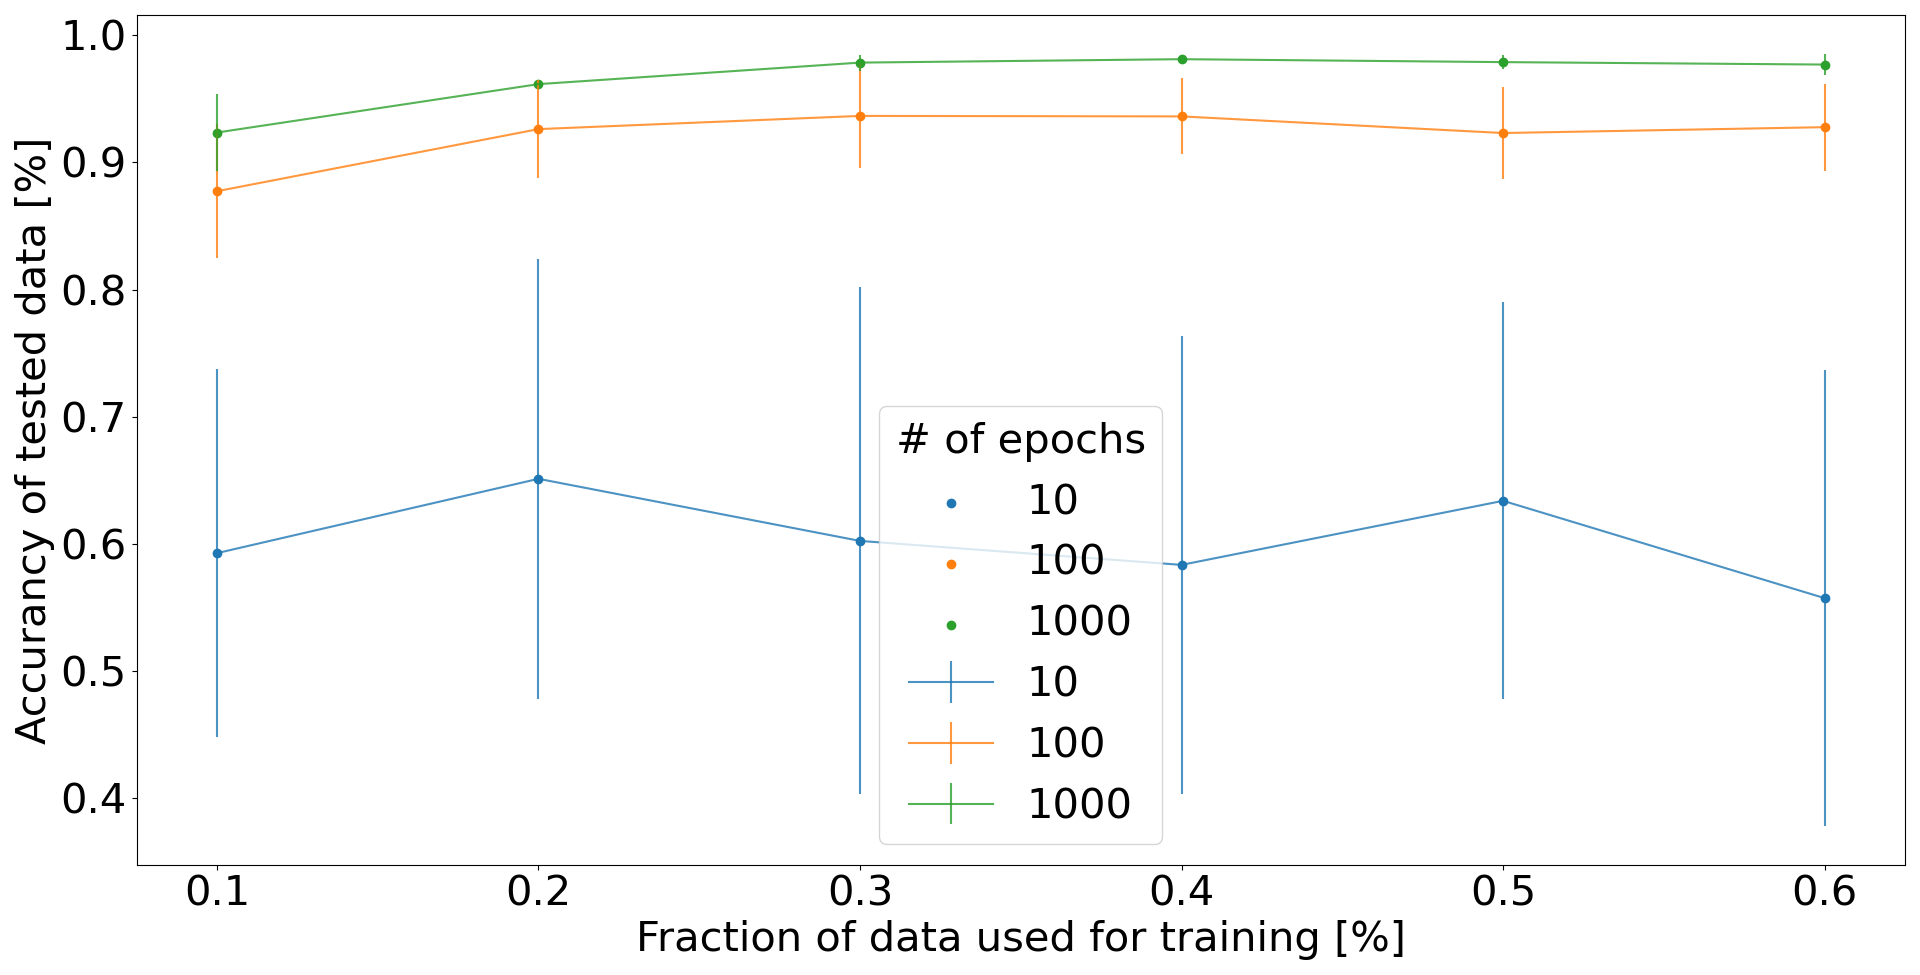
\includegraphics[width=\textwidth]{images/benchmark_nn.png}
\caption{Benchmark of the \texttt{WineDecision} NN.}
\label{fig:benchmark_nn}
\end{figure}

\section{Conclusion and Outlook}
In this introductory Propaedeuticum, the mathematical background and basic ideas of how NNs work were explained. In particular, the focus was on probabilistic considerations and advantages of using PyTorch to convey the basic idea. Details of results of the toy problem were deliberately not discussed, as they do not contribute to the topic of the actual bachelor thesis.
A NN approximates a posterior probability density function using a training data set by optimizing weights. PyTorch offers useful concepts and functions to avoid larger implementation efforts. In order to reproduce this work, code performing the described steps of the toy problem and the benchmark are available on GitHub \cite{Wine-Mining}.